\documentclass[11pt]{article}
\usepackage[margin=1in]{geometry}
\usepackage[T1]{fontenc}
\usepackage[utf8]{inputenc}
\usepackage{lmodern}
\usepackage{hyperref}
\usepackage{titlesec}
\usepackage{array}
\usepackage{longtable}
\usepackage{enumitem}
\usepackage{float}
\usepackage{forest}
\usepackage{amsmath}

\hypersetup{
  colorlinks=true,
  linkcolor=blue,
  urlcolor=blue
}
\setlength{\parskip}{0.5em}
\setlength{\parindent}{0pt}

% Turn off section numbering
\setcounter{secnumdepth}{-1}

% Optional styling
\titleformat{\section}{\large\bfseries}{}{0pt}{}
\titleformat{\subsection}{\normalsize\bfseries}{}{0pt}{}
\titleformat{\subsubsection}{\normalsize\bfseries}{}{0pt}{}

\begin{document}
\begin{center}
    {\LARGE \textbf{Delivery 2}}\\[0.5em]
\end{center}
\section{Task 1: Identifying and finding inconsistencies in the vision document}

\subsection{Defects table}

\small
\renewcommand{\arraystretch}{1.3}
\begin{longtable}{|c|p{2.3cm}|p{2cm}|p{1.5cm}|p{4.5cm}|c|c|}
\hline
\textbf{\#} & \textbf{Location} & \textbf{Defect Type} & \textbf{Class.} & \textbf{Description} & \textbf{Status} & \textbf{Date} \\
\hline
\endfirsthead

\multicolumn{7}{c}{\tablename\ \thetable{} -- continued from previous page} \\
\hline
\textbf{\#} & \textbf{Location} & \textbf{Defect Type} & \textbf{Class.} & \textbf{Description} & \textbf{Status} & \textbf{Date} \\
\hline
\endhead

\hline
\multicolumn{7}{r}{\textit{Continued on next page}} \\
\endfoot

\hline
\endlastfoot

1 & Sec. 3.4 vs. Sec. 5.1 & Omission & Major & There is a need ``Track spending and nutrition'' (Medium priority), but no feature exists to track grocery spending against the budget set, nor nutrition tracking. & Open & N/A \\
\hline

2 & Feature 14 (5.1) & Omission & Major & ``Historical Data Charts'' references calories eaten over past weeks, but no feature stores daily nutrition/calorie intake. & Open & N/A \\
\hline

3 & Feature 13 (5.1) vs. Sec. 4.1/6.2 & Contradiction & Major & Alerts/reminders to students' ``smart devices,'' suggests push notifications while Sec. 4.1/6.2 define Healthy Living strictly as a browser-based web app with alerting capabilities. & Open & N/A \\
\hline

4 & Features 9 \& 10 (5.1) & Ambiguity & Minor & ``Recipe Search and Filtering'' and ``Recipe Suggestions Based on Meal Plan'' can be  the same feature or two distinct mechanisms. Needs to be clarified. & Open & N/A \\
\hline

5 & Feature 20 (5.2) & Unmeasurability & Minor & ``Event Log Viewing'' has no measurable criteria, such as: retention period or granularity. & Open & N/A \\
\hline

6 & Feature 26 (5.3) & Opacity & Minor & ``Recipe View and Usage Reports'' doesn't explain why this belongs to the Content Moderator rather than another suitable role such as manager. & Open & N/A \\
\hline

\end{longtable}


\subsection{Inconsistencies table}


\small
\renewcommand{\arraystretch}{1.3}
\begin{longtable}{|c|p{2.6cm}|p{1.9cm}|p{1.3cm}|p{5.2cm}|c|c|}
\caption{Inconsistencies identified in the Vision Document} \\
\hline
\textbf{\#} & \textbf{Location} & \textbf{Inconsistency Type} & \textbf{Class.} & \textbf{Description} & \textbf{Status} & \textbf{Date} \\
\hline
\endfirsthead

\multicolumn{7}{c}{\tablename\ \thetable{} -- continued from previous page} \\
\hline
\textbf{\#} & \textbf{Location} & \textbf{Inconsistency Type} & \textbf{Class.} & \textbf{Description} & \textbf{Status} & \textbf{Date} \\
\hline
\endhead

\hline
\multicolumn{7}{r}{\textit{Continued on next page}} \\
\endfoot

\hline
\endlastfoot

1 & Sec. 1.1 with Features 7-8 & Terminology & Weak & \textbf{S1} Sec. 1.1 uses ``shopping list,'' while \textbf{S2} Feature 7 and Feature 8 uses ``grocery list'' for the same concept. The two terms seem interchangeable, so it is unclear if they denote the same thing. & Open & N/A \\
\hline

2 & Sec. 3.1 with Sec. 4.1 & Designation & Strong & \textbf{S3} Sec. 3.1 formally names the role ``System Administrator,'' but \textbf{S4} Sec. 4.1 shortens it to ``Administrator'' without explanation, creating confusion with a generic admin role. & Open & N/A \\
\hline

3 & Sec. 1 with Sec. 6.2& Terminology & Weak & \textbf{S5} Sec. 1 uses the term (``web-based application'') and \textbf{S6} Sec. 6.2 uses (``web app''), they both appear to refer to the same system, but no single term is established. & Open & N/A \\
\hline

4 & Sec. 6.1 with Features 21-23  & Terminology & Weak & \textbf{S7} Sec. 6.1 refers only to ``student data,'' while \textbf{S8} Features 21-23 distinguishes ``student'' data from ``recipe content'' owned by the Content Moderator. It is unclear whether S7's privacy standard also covers recipe metadata. & Open & N/A \\
\hline

5 & Feature 2 with Feature 9 & Terminology & Strong & \textbf{S9} (Sec. 5.1 Feature 2) indicates that student can save their diet, allergies and cooking skill while \textbf{S10} (Sec. 5.1, Feature 9) introduces filtering recipes by ingredients, difficulty and time, filter should be consistent with student preferences, only cooking skill/difficulty is similar & Open & N/A \\
\hline

\end{longtable}


\section{Task 2: Documenting conflicts}

\small
\renewcommand{\arraystretch}{1.3}
\begin{tabular}{|c|c|c|c|c|c|c|c|c|c|c|c|}
\hline
\textbf{Statement} & \textbf{S1} & \textbf{S2} & \textbf{S3} & \textbf{S4} & \textbf{S5} & \textbf{S6} & \textbf{S7} & \textbf{S8} & \textbf{S9} & \textbf{S10} & \textbf{Total} \\
\hline
S1  & 0 & 1000 & 0 & 0 & 0 & 0 & 0 & 0 & 0 & 0 & 1000 \\
\hline
S2  & 1000 & 0 & 0 & 0 & 0 & 0 & 0 & 0 & 0 & 0 & 1000 \\
\hline
S3  & 0 & 0 & 0 & 1000 & 0 & 0 & 0 & 0 & 0 & 0 & 1000 \\
\hline
S4  & 0 & 0 & 1000 & 0 & 0 & 0 & 0 & 0 & 0 & 0 & 1000 \\
\hline
S5  & 0 & 0 & 0 & 0 & 0 & 1000 & 0 & 0 & 0 & 0 & 1000 \\
\hline
S6  & 0 & 0 & 0 & 0 & 1000 & 0 & 0 & 0 & 0 & 0 & 1000 \\
\hline
S7  & 0 & 0 & 0 & 0 & 0 & 0 & 0 & 1 & 0 & 0 & 1 \\
\hline
S8  & 0 & 0 & 0 & 0 & 0 & 0 & 1 & 0 & 0 & 0 & 1 \\
\hline
S9  & 0 & 0 & 0 & 0 & 0 & 0 & 0 & 0 & 0 & 1 & 1 \\
\hline
S10 & 0 & 0 & 0 & 0 & 0 & 0 & 0 & 0 & 1 & 0 & 1 \\
\hline
\textbf{Total} & 1000 & 1000 & 1000 & 1000 & 1000 & 1000 & 1 & 1 & 1 & 1 & 6004 \\
\hline
\end{tabular}


\section{Task 3: Conflict Resolution}

\subsection*{Conflict Resolution: Inconsistency \#4 (S7 vs. S8)}

\begin{itemize}[leftmargin=1.5em]
  \item \textbf{S7} (Sec.~6.1): ``Data protection and privacy practices apply to student data.''
  \item \textbf{S8} (Features 21--23): Content Moderator features treat ``recipe content'' as a separate category, owned and managed independently from student data.
  \item \textbf{Conflict:} S7 is ambiguous whether recipe content (which may include user-submitted or user-rated data) falls under the same privacy protections as student data, since S8 implies recipe content is a distinct data classification.
\end{itemize}

\textbf{Resolution 1: Specialize conflict source or target:}
\begin{itemize}[leftmargin=1.5em]
  \item Split the single ``data'' object in S7 into two explicitly named subtypes: \textit{student personal data} (dietary preferences, allergies, budget, account info) and \textit{recipe/content data} (ingredients, steps, tags).
  \item Rewrite S7 as: ``Data protection and privacy practices apply to student personal data.''
  \item Add a new standard in Sec.~6.1: ``Content integrity and accuracy practices (not privacy practices) apply to recipe content, as recipe content is not personally identifiable.''
  \item This removes the ambiguity by giving each data type its own governing rule.
\end{itemize}

\textbf{Resolution 2: Weaken conflicting statements:}
\begin{itemize}[leftmargin=1.5em]
  \item Broaden S7 so it explicitly covers both categories instead of leaving recipe content unaddressed.
  \item Rewrite S7 as: ``Data protection and privacy practices apply to all data collected or generated within the system, including student personal data and any user-contributed recipe content (e.g., ratings, reviews) that could be linked back to a student.''
  \item This removes the conflict by making the privacy standard inclusive rather than just to ``student data.''
\end{itemize}

\subsection*{Conflict Resolution: Inconsistency \#5 (S9 vs. S10)}

\begin{itemize}[leftmargin=1.5em]
  \item \textbf{S9} (Feature 2): A student can save their diet, allergies and cooking skill so the app can suggest things that fit them.
  \item \textbf{S10} (Feature 9): A student can find recipes by ingredient, difficulty or time, but diet and allergy preferences are not listed as filter criteria, only ``difficulty'' loosely maps to ``cooking skill.''
  \item \textbf{Conflict:} Feature 9's filtering criteria don't fully align with the preference fields Feature 2 promises to use, so it's unclear whether saved diet/allergy preferences are actually applied when searching recipes.
\end{itemize}

\textbf{Resolution 1: Weaken conflicting statements:}
\begin{itemize}[leftmargin=1.5em]
  \item Relax Feature 9 so it doesn't have to be the sole search mechanism.
  \item Clarify that saved preferences from Feature 2 are applied as a separated automatic filter layered on top of manual search.
  \item Rewrite Feature 9 as: ``A student can find recipes by ingredient, difficulty, or time. Results are automatically pre-filtered by the student's saved diet and allergy preferences and can be further refined manually.''
  \item This removes the conflict by making the two features complementary rather than contradictory in scope.
\end{itemize}

\textbf{Resolution 2: Specialize conflict source or target:}
\begin{itemize}[leftmargin=1.5em]
  \item Specialize the ``filtering criteria'' object in Feature 9 into two distinct subsets: \textit{manual filters} (ingredient, difficulty, time) and \textit{profile-based filters} (diet, allergies).
  \item Rewrite Feature 9 as two clearly separated behaviors instead of one, so each filter type has its own defined source.
  \item This removes ambiguity about whether profile preferences are performed during search.
\end{itemize}

\section{Task 4: Conflict Evaluation}

\subsection*{Conflict \#4 (S7 vs. S8) -- Student Data vs. Recipe Content Privacy Scope}

Two alternatives were proposed to resolve this conflict.

\textbf{Alternative 1: Specialize conflict source or target:}
\begin{itemize}[leftmargin=1.5em]
  \item Splits ``data'' in S7 into two explicit subtypes: \textit{student personal data} and \textit{recipe/content data}, each governed by its own rule.
  \item Privacy practices apply only to student personal data, a different content-integrity rule applies to recipe content.
  \item Offers cleaner separation of concerns and it is easier for developers to understand.
  \item Requires more upfront design work to define and maintain two distinct data-governance categories.
\end{itemize}

\textbf{Alternative 2: Weaken conflicting statements:}
\begin{itemize}[leftmargin=1.5em]
  \item Broadens S7's scope so privacy practices apply to \textit{all} data in the system, including any recipe content that could be linked back to a student.
  \item Removes the ambiguity by making the rule maximally inclusive rather than precisely scoped.
  \item Simpler to state and closes all compliance gaps by default.
  \item Imposes privacy overhead on data that does not require it.
\end{itemize}

\begin{table}[H]
\centering
\small
\renewcommand{\arraystretch}{1.3}
\begin{tabular}{|p{4cm}|c|c|c|}
\hline
\textbf{Evaluation Criteria} & \textbf{Weight} & \textbf{Alt. 1 (Specialize)} & \textbf{Alt. 2 (Weaken)} \\
\hline
Regulatory / privacy compliance robustness & 0.4 & 4 & 5 \\
\hline
Ease of implementation & 0.3 & 3 & 4 \\
\hline
Infrastructure cost & 0.3 & 4 & 2 \\
\hline
\hline
\textbf{Weighted Total} & 1.0 & \textbf{3.7} & \textbf{3.8} \\
\hline
\end{tabular}
\end{table}

\textbf{Winner: Alternative 2 (Weaken conflicting statements).} Broadening S7's scope achieves the highest compliance robustness, but this advantage is partly offset by its higher infrastructure cost, since applying privacy-grade controls (encryption, access restrictions) to all data, including recipe content, requires a larger investment than protecting only student personal data. If infrastructure budget were a harder constraint for the project, Alternative 1 (Specialize conflict source or target) would be the more cost-effective choice, since it limits protections to the smaller, higher-risk data subset.

\subsection*{Conflict \#5 (S9 vs. S10) -- Preference Storage vs. Recipe Filtering}

Two alternatives were proposed to resolve this conflict.

\textbf{Alternative 1: Weaken conflicting statements:}
\begin{itemize}[leftmargin=1.5em]
  \item Layers saved diet and allergy preferences from Feature 2 automatically on top of manual search.
  \item Results are pre-filtered by profile data and can be further refined by the student.
  \item Delivers a more seamless, single-step experience for the student.
  \item Reuses the existing user-profile filter logic, reducing duplicated code to maintain.
\end{itemize}

\textbf{Alternative 2: Specialize conflict source or target:}
\begin{itemize}[leftmargin=1.5em]
  \item Specializes ``filtering criteria'' into two distinct subsets: \textit{manual filters} (ingredient, difficulty, time) and \textit{profile-based filters} (diet, allergies).
  \item Rewrites Feature 9 as two clearly separated functionalities instead of one.
  \item Simpler to implement, easier to test each mechanism in isolation.
  \item Risks code duplication and drift, since allergen/diet filtering will be implemented separately.
\end{itemize}

\begin{table}[H]
\centering
\small
\renewcommand{\arraystretch}{1.3}
\begin{tabular}{|p{4cm}|c|c|c|}
\hline
\textbf{Evaluation Criteria} & \textbf{Weight} & \textbf{Alt. 1 (Weaken)} & \textbf{Alt. 2 (Specialize)} \\
\hline
User experience / personalization accuracy & 0.4 & 5 & 4 \\
\hline
Implementation complexity & 0.3 & 3 & 4 \\
\hline
Maintainability & 0.3 & 5 & 2 \\
\hline
\hline
\textbf{Weighted Total} & 1.0 & \textbf{4.4} & \textbf{3.4} \\
\hline
\end{tabular}
\caption{Evaluation of alternatives for Conflict \#5 (scale 1--5, weighted score = $\sum$ weight $\times$ score)}
\end{table}

\textbf{Winner: Alternative 1 (Weaken conflicting statements).} Alternative 1 wins clearly (4.4 vs. 3.4). Layering saved diet and allergy preferences on top of manual search keeps allergen and dietary logic in a single, reusable code path shared with the rest of the user-profile system, rather than duplicating similar filtering logic across two separate mechanisms. While Alternative 2 (Specialize conflict source or target) offers slightly better implementation complexity in isolation, the long-term maintenance burden of keeping duplicated filter logic consistent with the main profile system outweighs that short-term benefit, making Alternative 1 the better choice.

\section{Task 5: Risk Management}

\subsection{a) Risk Identification}

\subsubsection{1. Component Inspection}

\begin{longtable}{|c|p{2.3cm}|p{2cm}|p{4.5cm}|p{3cm}|}
\hline
\textbf{ID} & \textbf{Component} & \textbf{Risk Category} & \textbf{Risk Description} & \textbf{Potential Impact} \\
\hline
\endfirsthead

\hline
\textbf{ID} & \textbf{Component} & \textbf{Risk Category} & \textbf{Risk Description} & \textbf{Potential Impact} \\
\hline
\endhead

\hline
\endfoot

\hline
\endlastfoot

R1 & Backend infrastructure & Hardware failure & Cloud provider or data center outage. & System-wide downtime at scale. \\
\hline

R2 & Student UI (client devices) & Hardware failure & Low-end student devices fail to render the app reliably. & Inconsistent access for some students. \\
\hline

R3 & All UIs & Network failure & Users connect from unstable or restricted networks (mobile, office, VPN). & Slow responses, dropped sessions, delayed staff actions. \\
\hline

R4 & Third-party nutrition/ingredient APIs & Network / External service failure & API downtime, connectivity issues, license expiration, or stricter rate limits/costs as usage scales. & Inaccurate or unavailable nutrition/recipe data. \\
\hline

\end{longtable}


\subsubsection{2. Risk Checklist}

\begin{enumerate}[leftmargin=1.7em]
  \item \textbf{Data confidentiality:} The app stores sensitive student data, including allergies, diet and budget information. Weak access controls, unencrypted storage or overly broad staff permissions could expose this data, creating both safety and privacy risks.

  \item \textbf{Usability:} Students with limited cooking skill and time need the app to feel simple and guided. There is a risk that meal planning, grocery and recipe features are too complex and that accessibility needs are not met.

  \item \textbf{Performance:} The app targets fast response times even on slow connections, while scaling to a large user base. Heavy reliance on third-party APIs and a shared database could cause slowdowns as usage grows.
\end{enumerate}

\subsubsection{3. Risk Tree}

\begin{figure}[H]
    \centering
    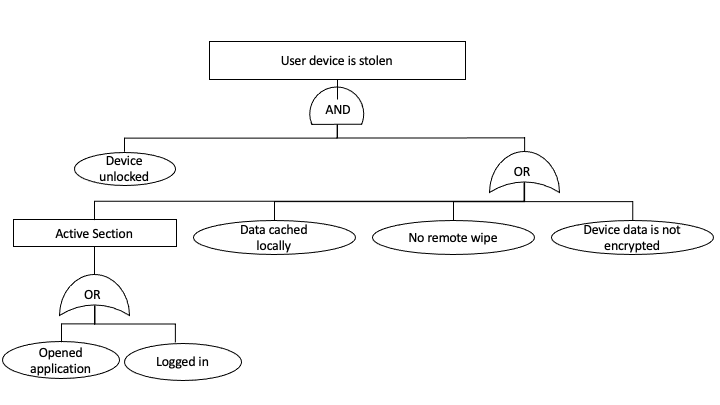
\includegraphics[width=0.9\textwidth]{images/risk-tree.png}
    \label{fig:risk-tree}
\end{figure}

\subsection{b) Risk Quantitative Assessment}

\begin{longtable}{|p{2.8cm}|p{4.5cm}|c|c|c|}
\hline
\textbf{Risk} & \textbf{Rationale} & \textbf{Likelihood} & \textbf{Severity} & \textbf{Risk Exposure} \\
\hline
\endfirsthead

\hline
\textbf{Risk} & \textbf{Rationale} & \textbf{Likelihood} & \textbf{Severity} & \textbf{Risk Exposure} \\
\hline
\endhead

\hline
\endfoot

\hline
\endlastfoot

Backend infrastructure outage & Cloud/data center outages are rare for major providers with SLA guarantees, but not impossible. & 5\% & 9 & 0.45 \\
\hline

Client device limitations & A good share of students use older or low-end devices, but most modern browsers still render web apps without issues. & 20\% & 4 & 0.80 \\
\hline

Unstable/restricted network access & Students and staff routinely connect from varied networks (mobile, home, office, VPN), hence some degree of slowness is expected regularly. & 40\% & 5 & 2.00 \\
\hline

Third-party API failure & External APIs occasionally have downtime, rate limits or schema changes. & 25\% & 6 & 1.50 \\
\hline

Data confidentiality breach & Requires a specific failure (weak access control, misconfiguration or attack). It is less likely if standard practices are followed, but high-impact if it occurs. & 10\% & 9 & 0.90 \\
\hline

Usability shortfalls & Complex features or accessibility gaps are a common risk in early releases, especially for a broad and time-constrained user base. & 30\% & 5 & 1.50 \\
\hline

Performance degradation under load & Meeting a strict 100ms target while scaling to millions of users is a realistic risk as adoption grows, especially with database/API dependencies. & 35\% & 6 & 2.10 \\
\hline

Stolen device with exposed data & Device theft is a plausible real-world event, though it requires additional conditions (no lock, active session) to result in actual data exposure. & 15\% & 8 & 1.20 \\
\hline

\end{longtable}

\subsection{c) Risk Control}

For each risk identified in the quantitative assessment, all viable countermeasures were listed and evaluated. When more than one alternative existed, the Risk Reduction Leverage (RRL) technique was applied to select the most cost-effective option:

$RRL = (RE_{\text{before}} - RE_{\text{after}}) / Cost$ 

Where cost is rated on a relative 1--3 scale (1 = low, 2 = medium, 3 = high). The countermeasure with the highest RRL was selected.

\subsubsection*{Backend infrastructure outage (Tactic: Reduce likelihood)}
\begin{itemize}[leftmargin=1.5em]
  \item \textbf{Countermeasure A: Proactive monitoring and alerting:}
  \begin{itemize}[leftmargin=1.5em]
    \item $RE_{\text{before}} = 0.45$, $RE_{\text{after}} = 0.27$, $Cost = 1$
    \item $RRL = (0.45 - 0.27) / 1 = 0.18$
  \end{itemize}
  \item \textbf{Countermeasure B: Multi-region failover:}
  \begin{itemize}[leftmargin=1.5em]
    \item $RE_{\text{before}} = 0.45$, $RE_{\text{after}} = 0.09$, $Cost = 3$
    \item $RRL = (0.45 - 0.09) / 3 = 0.12$
  \end{itemize}
  \item \textbf{Selected: Countermeasure A} (RRL 0.18 $>$ 0.12). Monitoring reduces exposure to \textbf{0.27} at the lowest cost. Failover offers a larger absolute reduction but at 3$\times$ the cost.
\end{itemize}

\subsubsection*{Client device limitations (Tactic: Reduce likelihood)}
\begin{itemize}[leftmargin=1.5em]
  \item \textbf{Countermeasure A: Responsive, progressively-enhanced UI tested on low-end devices:}
  \begin{itemize}[leftmargin=1.5em]
    \item $RE_{\text{before}} = 0.80$, $RE_{\text{after}} = 0.40$, $Cost = 1$
    \item $RRL = (0.80 - 0.40) / 1 = 0.40$
  \end{itemize}
  \item \textbf{Countermeasure B: Lightweight fallback mode for low-end devices:}
  \begin{itemize}[leftmargin=1.5em]
    \item $RE_{\text{before}} = 0.80$, $RE_{\text{after}} = 0.40$, $Cost = 2$
    \item $RRL = (0.80 - 0.40) / 2 = 0.20$
  \end{itemize}
  \item \textbf{Selected: Countermeasure A} (RRL 0.40 $>$ 0.20). Both countermeasures achieve the same exposure reduction to \textbf{0.40}, but responsive design testing costs half.
\end{itemize}

\subsubsection*{Unstable/restricted network access (Tactic: Mitigate consequence)}
\begin{itemize}[leftmargin=1.5em]
  \item \textbf{Countermeasure A: Retry logic and optimistic UI updates:}
  \begin{itemize}[leftmargin=1.5em]
    \item $RE_{\text{before}} = 2.00$, $RE_{\text{after}} = 1.20$, $Cost = 1$
    \item $RRL = (2.00 - 1.20) / 1 = 0.80$
  \end{itemize}
  \item \textbf{Countermeasure B: Offline-first caching via a service worker:}
  \begin{itemize}[leftmargin=1.5em]
    \item $RE_{\text{before}} = 2.00$, $RE_{\text{after}} = 1.25$, $Cost = 2$
    \item $RRL = (2.00 - 1.25) / 2 = 0.375$
  \end{itemize}
  \item \textbf{Selected: Countermeasure A} (RRL 0.80 $>$ 0.375). Retry logic achieves both a larger reduction (to \textbf{1.20} vs. 1.25) and a lower cost than offline caching.
\end{itemize}

\subsubsection*{Third-party API failure (Tactic: Reduce likelihood)}
\begin{itemize}[leftmargin=1.5em]
  \item \textbf{Countermeasure A: Select providers with strong SLAs and add uptime monitoring:}
  \begin{itemize}[leftmargin=1.5em]
    \item $RE_{\text{before}} = 1.50$, $RE_{\text{after}} = 0.90$, $Cost = 1$
    \item $RRL = (1.50 - 0.90) / 1 = 0.60$
  \end{itemize}
  \item \textbf{Countermeasure B: Cache nutrition data locally as a fallback:}
  \begin{itemize}[leftmargin=1.5em]
    \item $RE_{\text{before}} = 1.50$, $RE_{\text{after}} = 0.75$, $Cost = 2$
    \item $RRL = (1.50 - 0.75) / 2 = 0.375$
  \end{itemize}
  \item \textbf{Selected: Countermeasure A} (RRL 0.60 $>$ 0.375). SLA selection and monitoring is more cost-effective.
\end{itemize}

\subsubsection*{Data confidentiality breach (Tactic: Avoid risk)}
\begin{itemize}[leftmargin=1.5em]
  \item \textbf{Countermeasure A: Role-based access control and encryption at rest/in transit:}
  \begin{itemize}[leftmargin=1.5em]
    \item $RE_{\text{before}} = 0.90$, $RE_{\text{after}} = 0.27$, $Cost = 2$
    \item $RRL = (0.90 - 0.27) / 2 = 0.315$
  \end{itemize}
  \item \textbf{Countermeasure B: Data anonymization/pseudonymization:}
  \begin{itemize}[leftmargin=1.5em]
    \item $RE_{\text{before}} = 0.90$, $RE_{\text{after}} = 0.50$, $Cost = 2$
    \item $RRL = (0.90 - 0.50) / 2 = 0.20$
  \end{itemize}
  \item \textbf{Selected: Countermeasure A} (RRL 0.315 $>$ 0.20). RBAC plus encryption achieves a much larger reduction to \textbf{0.27} at the same cost and directly satisfies the data protection standard already required for the product.
\end{itemize}

\subsubsection*{Usability shortfalls (Tactic: Reduce likelihood)}
\begin{itemize}[leftmargin=1.5em]
  \item \textbf{Countermeasure A: Usability testing with representative students before release:}
  \begin{itemize}[leftmargin=1.5em]
    \item $RE_{\text{before}} = 1.50$, $RE_{\text{after}} = 0.75$, $Cost = 1$
    \item $RRL = (1.50 - 0.75) / 1 = 0.75$
  \end{itemize}
  \item \textbf{Selected: Countermeasure A}. Only one credible countermeasure was identified. It directly targets the root cause at low cost, so no RRL comparison against a second alternative was required.
\end{itemize}

\subsubsection*{Performance degradation under load (Tactic: Mitigate consequence)}
\begin{itemize}[leftmargin=1.5em]
  \item \textbf{Countermeasure A: Graceful degradation (serve cached responses or reduced feature set under heavy load):}
  \begin{itemize}[leftmargin=1.5em]
    \item $RE_{\text{before}} = 2.10$, $RE_{\text{after}} = 1.05$, $Cost = 1$
    \item $RRL = (2.10 - 1.05) / 1 = 1.05$
  \end{itemize}
  \item \textbf{Countermeasure B: Load testing with horizontal auto-scaling:}
  \begin{itemize}[leftmargin=1.5em]
    \item $RE_{\text{before}} = 2.10$, $RE_{\text{after}} = 1.20$, $Cost = 2$
    \item $RRL = (2.10 - 1.20) / 2 = 0.45$
  \end{itemize}
  \item \textbf{Selected: Countermeasure A} (RRL 1.05 $>$ 0.45). Graceful degradation achieves a larger reduction (to \textbf{1.05} vs. 1.20) at half the cost of auto-scaling.
\end{itemize}

\subsubsection*{Stolen device with exposed data (Tactic: Reduce consequence likelihood)}
\begin{itemize}[leftmargin=1.5em]
  \item \textbf{Countermeasure A: Automatic session timeout and mandatory re-authentication for sensitive actions:}
  \begin{itemize}[leftmargin=1.5em]
    \item $RE_{\text{before}} = 1.20$, $RE_{\text{after}} = 0.60$, $Cost = 1$
    \item $RRL = (1.20 - 0.60) / 1 = 0.60$
  \end{itemize}
  \item \textbf{Countermeasure B: Remote logout/device deactivation feature:}
  \begin{itemize}[leftmargin=1.5em]
    \item $RE_{\text{before}} = 1.20$, $RE_{\text{after}} = 0.45$, $Cost = 2$
    \item $RRL = (1.20 - 0.45) / 2 = 0.375$
  \end{itemize}
  \item \textbf{Selected: Countermeasure A} (RRL 0.60 $>$ 0.375). Session timeout with re-authentication achieves stronger protection at lower cost. Remote logout remains a valuable complementary feature but is not the most cost-effective.
\end{itemize}


\section{Appendix}

\begin{longtable}{|p{8cm}|c|}
\hline
\textbf{Section} & \textbf{Duration (hours)} \\
\hline
\endfirsthead

\hline
\textbf{Section} & \textbf{Duration (hours)} \\
\hline
\endhead

\hline
\endfoot

\hline
\endlastfoot

Task 1 -- Identifying and finding inconsistencies in the vision document & 4 \\
\hline
Task 2 -- Documenting conflicts & 3 \\
\hline
Task 3 -- Conflict resolution & 3 \\
\hline
Task 4 -- Conflict evaluation & 4 \\
\hline
Task 5 -- Risk management & 5 \\
\hline

\end{longtable}

\end{document}